\chapter{绪论}
\label{chap:introduction}

本章的内容包括对当前快速进步、扩张、提升下的互联网里对于实体关系的知识抽取调研的背景以及意义,阐释了在当先信息大爆炸的互联网时代里,通过从不计其数的信息中提取出实体,之后以实体之间关系的知识抽取对建立全面而准确的信息知识数据库,从而更好地服务互联网的使用者。

也包括了介绍国内外对于本课题的研究现状和本文的研究内容。

\section{研究背景与意义}
\subsection{研究背景}

传统的信息提取涉及很多人为因素的干扰,包括手工制定的规则或手工标注出来的样例来作为机器学习的输入数据,从而识别并判断在文本中两个实体之间的特定关系\citep{wang}。即使机器学习可以帮助枚举出潜在的可供提取的关系模式,但这个方式常常受制于提取已经被预定义的关系集。并且,这个方式不能适用于如今充斥着大量信息的互联网,特别是非结构化、未预先定义实体关系的信息。

另一种开放的信息抽取\citep{banko}方式独立于关系领域,从文本抽取关系并能方便地度量网络语料库的多样性和覆盖范围。语料库是开放式信息抽取系统所需要的唯一一种输入数据,它的输出是被抽取出的各种关系的集合。一个开放式信息抽取系统通过它的语料库大小来控制它所能抽取关系的可扩展性,并用以下方法来增加可处理的关系类型:基于浅分析、基于语法或没有预定义关系的基于词法分析的模式匹配\citep{wu2010, naka2012, etz2011}。现在的开放式关系抽取技术主要关注字面上关系的抽取,而没有尝试进行词法分析,但词法分析却是传统信息抽取的优点。

\subsection{研究意义}
ZORE 外的其他的开放式关系抽取系统是抽取二元的关系,之后将其归纳为语义模式。而 ZORE 则同时进行抽取关系和归纳模式,利用双重拓展的算法让关系和模式信息互相加固加强,从而减弱自动词法分析和自动语义分析所带来的负面影响,语义模式信息可以对提升关系抽取带来帮助。所以本次毕设采用了 ZORE 做为关系抽取的引擎。

\section{开放式关系抽取的基本定义}
ZORE 是被应用于网络文本来提取普遍意义上的关系和它们的语义类型。对于关系的定义大部分都是来自于英文语境下,但是此次毕设的语义环境处在中文里,所以需要对这种特定语言的开放式关系抽取进行一些中文语境下的调整。以下的解释以句子“侯建国校长就职于中国科学技术大学”做为样例。

\begin{figure}[ht]
\centering
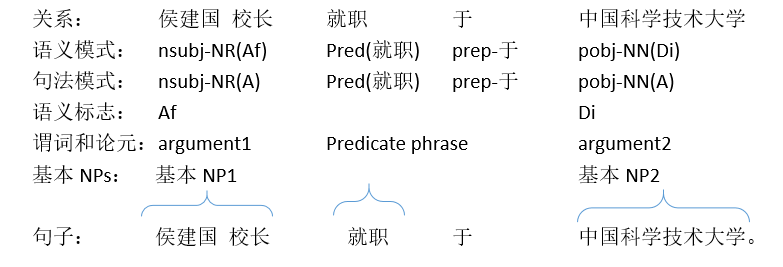
\includegraphics[width=15cm]{sentence1}
\caption{分析样例句子}\label{fig:sentence1}
\end{figure}

\subsection{预测短语(predicate phrase)}
预测短语是包括至少一个动词或系词,并在语句构成上控制至少一个名词的词语序列。例如,图 1.1 里的预测短语是“就职”。为了预防“少动词结构”的情况出现,动词和它所直接“控制”的对象共同被认为是一个“预测短语”。介词并不被包括在预测短语的范围中。

\subsection{参数(argument)}
参数是一个被预测短语所直接控制或通过介词间接控制的基本名词短语。例如,图 1.1 里的“侯建国校长”和“中国科学技术大学”就是预测短语“就职”的两个参数。

\subsection{关系(relation)}
一个“二元关系”是一个包括了预测短语 pred 和它的两个参数 x 与 y 的三元组。依此类推,一个“n 元关系”则包括了 n 个参数。例如,图 1.1 里的句子包含了一个二元关系(x[侯建国校长], pred[就职], y[中国科学技术大学])。在英文语境下,二元关系的两个参数通常分别位于 pred 的左边和右边。因此,弱模式对于英文语境下的的关系抽取非常有效。然而在中文语境下,二元关系的两个关系有可能都在 pred 的左边(例如“我和你打架”),都在 pred 的右边(例如“抄袭了我的作业”),或者一左一右分布在 pred 的两边,即根据不同的句子,出现的关系模式可能为(x, y, pred),(pred, x, y)和(x, pred, y)。从而让关系短语的探测变得更加复杂。

\subsection{句法模式(syntactic pattern)}
